\documentclass{spbau-diploma}

% пакеты
\usepackage{amsthm}
\usepackage{amssymb}
% \usepackage{mdsymbol}
\usepackage{mathtools}
\usepackage{algorithm}
\usepackage[singlelinecheck=false,justification=justified]{caption}
\usepackage{algorithmicx}
\usepackage[noend]{algpseudocode}
\usepackage{tikz}
\usetikzlibrary{fit,automata,positioning}
\usetikzlibrary{decorations.pathmorphing}
\tikzset{
  snake it/.style={decorate, decoration=snake},
  every state/.style={minimum size=0.3cm}}
\usepackage[normalem]{ulem}

\usepackage{perpage}
\MakePerPage{footnote}
% \renewcommand{\thefootnote}{\fnsymbol{footnote}}

% Основные математические символы
\def\eps{\varepsilon}                  % eps
\def\oo{\infty}                        % oo
\def\SO{\Rightarrow}                   % =>
\def\EQ{\Leftrightarrow}               % <=>
\def\t{\texttt}                        % mono font
\def\s{\textsc}                        % small capitals (for problem names)
\def\c#1{{\rm\sc{#1}}}                 % font for classes \t{NP} etc
\def\O{\mathcal{O}}                    % cool big O
\def\NO{\t{\#}}                        % #
\def\edge{\leftrightarrow}             % <->
\def\to{\rightarrow}                   % ->
\def\path{\rightsquigarrow}            % ~~>
\def\su{\sum\limits}                   % sum
\renewcommand{\le}{\leqslant}          % <=, beauty
\renewcommand{\ge}{\geqslant}          % >=, beauty
\newcommand{\q}[1]{\langle #1 \rangle} % <x>
\newcommand{\cool}[1]{\mathcal{#1}}    % fancy letters

\def\TODO{{\color{red}{\bf TODO}}}

\newtheorem{theorem}{Теорема}[section]
\newtheorem{lemma}{Лемма}[section]
\newtheorem{example}{Пример}[section]
\newtheorem{proposition}{Утверждение}[section]
\newtheorem{corollary}{Следствие}[theorem]

\theoremstyle{remark}
\newtheorem*{remark}{Замечание}
\newtheorem*{note}{Замечание}

\theoremstyle{definition}
\newtheorem{definition}{Определение}[section]

\begin{document}
% Год, город, название университета и факультета предопределены,
% но можно и поменять.
% Если англоязычная титульная страница не нужна, то ее можно просто удалить.
\filltitle{ru}{
    chair              = {Кафедра математических и информационных технологий},
    title              = {Пустое подмножество как замкнутое множество},
    % Здесь указывается тип работы. Возможные значения:
    %   coursework - Курсовая работа
    %   diploma - Диплом специалиста
    %   master - Диплом магистра
    %   bachelor - Диплом бакалавра
    type               = {master},
    position           = {студента},
    group              = 666,
    author             = {Машкин Эдельвейс Захарович},
    supervisorPosition = {д.\,ф.-м.\,н., профессор},
    supervisor         = {Выбегалло А.\,А.},
    reviewerPosition   = {ст. преп.},
    reviewer           = {Привалов А.\,И.},
    chairHeadPosition  = {д.\,ф.-м.\,н., профессор},
    chairHead          = {Омельченко А.\,В.},
    % university = {САНКТ-ПЕТЕРБУРГСКИЙ АКАДЕМИЧЕСКИЙ УНИВЕРСИТЕТ},
    % faculty = {Центр высшего образования},
    % city = {Санкт-Петербург},
    % year             = {2013}
}
\filltitle{en}{
    chair              = {Department of Mathematics and Information Technology},
    title              = {Empty subset as closed set},
    author             = {Edelweis Mashkin},
    supervisorPosition = {professor},
    supervisor         = {Amvrosy Vibegallo},
    reviewerPosition   = {assistant},
    reviewer           = {Alexander Privalov},
    chairHeadPosition  = {professor},
    chairHead          = {Alexander Omelchenko},
}
\maketitle
\tableofcontents

% \section*{Аннотация}

\textit{Задача поиска путей с контекстно-свободными ограничениями} является одной из важных задач в работе с графовыми моделями данных. Создано множество алгоритмов для её решения, но все они недостаточно эффективны для применения на практике, так что разрабатываются частные решения, более оптимальные, чем общие. Однако существующие частные решения слишком разнородны и не могут быть переиспользованы для построения новых алгоритмов. В данной работе был предложен общий подход к созданию эффективных частных решений, заключающийся в модификациях алгоритма, основанного на идее пересечения языков и поддержке инкрементального транзитивного замыкания. Одной из таких модификаций является работа с неориентированными графами вместо ориентированных. Полученный с её помощью алгоритм применим для решения задачи поиска путей с контекстно-свободными ограничениями на двунаправленных графах и языке Дика. Вторая модификация заключается в пересчёте транзитивного замыкания после каждой итерации добавления рёбер, вместо поддержки обновления отношения достижимости при одиночном добавлении. Такое решение применимо при малом числе итераций пересчёта транзитивного замыкания. Для языка Дика на одном типе скобок была сконструирована специальная грамматика, дающее полилогарифмическое число итераций и, следовательно, субкубический алгоритм. Также идея пересечения языков была использована для ускорения решения другой задачи, а именно, поиска путей с ограничениями, заданными смешанным языком Дика.

\vspace{1em}

\textit{Ключевые слова:} задача достижимости, графовые алгоритмы, формальные языки, транзитивное замыкание, частные случаи

\pagebreak

\textit{Context-free path querying problem} is an important task for graph­based data models. Many algorithms for this problem have been proposed, but none of them is performant enough for practical use, so more effective solutions for special cases are being developed. However, the existing partial solutions are too diverse and cannot be reused to build new algorithms. In this work, we propose a general approach for creating effective partial solutions, based on the idea of language intersection and incremental transitive closure. Each partial solution is a modification of the baseline algorithm. One such modification is to consider undirected graphs instead of directed one. This modification can be applied to bidirected graphs and Dyck language. The second modification is to recalculate the transitive closure after each iteration of edge additions, instead of incremental updating of reachability relation. This solution is effective on graphs with a small number of transitive closure recalculation iterations. For Dyck language with one parenthesis type special grammar was constructed, such that number of iterations of transitive closure recalculation is poly\-logarithmic, which implies a subcubic algorithm. Also, the idea of language intersection was used to speed up the solution for another problem, that is paths querying with constraints given by interleaved Dyck language.

\vspace{1em}

\textit{Keywords:} reachability problem, graph algorithms, formal languages, transitive closure, special cases
\section*{Введение}

\subsection*{Актуальность}

Графовые модели данных широко используются в различных областях науки, например, в биоинформатике~\cite{Sevon08}, анализе социальных сетей~\cite{Zarrinkalam14, Chaudhary16}, графовых базах данных~\cite{Medeiros18,Yannakakis1990} и разных видах статического анализа~\cite{Reps1998}. 

Одной из важных задач в анализе графовых моделей данных является поиск путей с заданными ограничениями. Одним из способов задавать такие ограничения являются формальные языки: если на рёбрах графа написаны метки из фиксированного алфавита, то можно искать пути, конкатенация меток на которых принадлежит фиксированному языку~\cite{Barrett00}. Например, хорошо изучена задача поиска путей с ограничениями, заданными регулярными языками~\cite{Mendelzon1995}. В этой же работе мы остановимся на классе контекстно-свободных языков, так как они позволяют решать более широкий класс задач.

Задача поиска путей с контекстно-свободными ограничениями, или, сокращённо, CFPQ\footnote{Context-Free Path Querying} была впервые сформулирована в терминах запросов к графовым базам данных~\cite{Yannakakis1990}, но нашла применение и в прочих отраслях, использующих графовые модели. За более чем 30 лет, прошедших с тех пор, было предложено множество разных алгоритмов для её решения~\cite{Reps97, Hellings15, Santos18}, в большинстве своём основанных на различных методах синтаксического анализа. 

К сожалению, все существующие решения задачи в общем случае недостаточно эффективны для использования на практике~\cite{Kuijpers19}. Более того, существует условная нижная оценка~\cite{Heintze1997}, согласно которой, скорее всего, достаточно быстрых решений задачи CFPQ в общем случае и не существует.

Всё вышесказанное приводит к тому, что имеет смысл разрабатывать алгоритмы для частных случаев задачи, имеющие время работы лучше, чем общее решение. Для некоторых из этих случаев уже были построены подобные решения, например для языков Дика на двунаправленных графах~\cite{Yuan09,Chatterjee17}. Проблема существующих решений в том, что они слишком Ad hoc, то есть построены специально под конкретный частный случай, а потому применённые в них подходы и идеи невозможно переиспользовать при построении решений для других частных случаев.  

Данная работа нацелена на создание единого подхода к построению решений задачи для CFPQ и применение этого подхода для разработки на его основе новых решений для некоторых частных случаев задачи.

\subsection*{Постановка задачи}

% Помеченный граф
\begin{definition}
  \textit{Ориентированный помеченный граф} (или \textit{граф с метками})~--- это тройка $G = \q{V, E, \Sigma}$, где $V$~--- множество вершин, $\Sigma$~--- множество меток, \\$E \subseteq V \times V \times \Sigma$~--- множество рёбер. 

  Неформально, это мультиграф, каждому ребру которого сопоставлена метка из алфавита $\Sigma$.
\end{definition}

\begin{figure}[H]
  \begin{minipage}[h]{0.5\linewidth}
    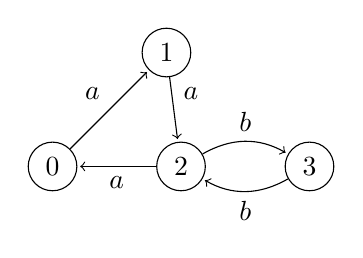
\begin{tikzpicture}[shorten >=1pt, auto]
      \node[state] (q_0)                      {$0$};
      \node[state] (q_1) [above right=of q_0] {$1$};
      \node[state] (q_2) [right=of q_0]       {$2$};
      \node[state] (q_3) [right=of q_2]       {$3$};
      \path[->]
        (q_0) edge node {$a$} (q_1)
        (q_1) edge node {$a$} (q_2)
        (q_2) edge node {$a$} (q_0)
        (q_2) edge[bend left, above]  node {$b$} (q_3)
        (q_3) edge[bend left, below]  node {$b$} (q_2);
    \end{tikzpicture}
    \caption{Помеченный граф с $\Sigma = \{ a, b \}$}
  \end{minipage}
  \hfill
  \begin{minipage}[h]{0.5\linewidth} 
      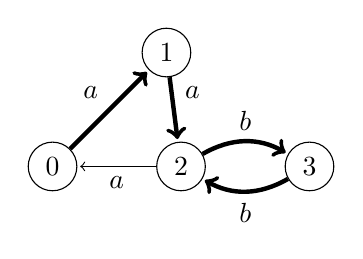
\begin{tikzpicture}[shorten >=1pt, auto]
        \node[state] (q_0)                      {$0$};
        \node[state] (q_1) [above right=of q_0] {$1$};
        \node[state] (q_2) [right=of q_0]       {$2$};
        \node[state] (q_3) [right=of q_2]       {$3$};
        \path[->]
          (q_0) edge[ultra thick] node {$a$} (q_1)
          (q_1) edge[ultra thick] node {$a$} (q_2)
          (q_2) edge node {$a$} (q_0)
          (q_2) edge[bend left, above, ultra thick]  node {$b$} (q_3)
          (q_3) edge[bend left, below, ultra thick]  node {$b$} (q_2);
      \end{tikzpicture}
      \caption{На пути $v_0 \to v_1 \to v_2 \to v_3 \to v_2$\\ читается слово $aabb$}
    \end{minipage}
    \label{tikz:labeled_graph}
\end{figure}


\begin{definition}
  Будем говорить, что слово $w$ \textit{читается} на пути $p$, если конкатенация меток вдоль $p$ образует $w$. 
\end{definition}

% Контекстно-свободная грамматика
\begin{definition}
  \textit{Контекстно-свободная грамматика}~--- это четвёрка $\q{\Sigma, N, S, P}$:
  \vspace{-\topsep}
  \begin{itemize}
    \setlength\itemsep{-0.1em}
    \item $\Sigma$~--- конечный алфавит
    \item $N$~--- конечное множество нетерминалов
    \item $S \in N$~--- стартовый нетерминал
    \item $P$~--- конечное множество продукций (правил вывода), имеющих вид\\ $N_i \to \alpha$, где $N_i \in N, \alpha \in (\Sigma \cup N)^{*}$
  \end{itemize}

  Язык, распознаваемый грамматикой $\cool{G}$~--- язык $L(G)$ слов, выводимых из стартового нетерминала.

  Контекстно-свободная грамматика задаёт \textit{контекстно-свободный язык}.
\end{definition}

\begin{example}
  Опишем грамматику $\cool{G} = \q{\Sigma, N, S, P}$, задающую язык $L(\cool{G})$ слов вида $b^n a^m b^{2n}$

  Алфавит состоит из букв $a$ и $b$: $\Sigma = \{ a, b \}$, нетерминалов будет два: $S$~-- стартовый нетерминал и $A$~--- нетерминал для слов вида $a^m$. Также вывода слов в грамматике будут следующие продукции:

  \begin{align*}
    &S \to b S bb \\
    &S \to A \\
    &A \to a A \\
    &A \to \eps
  \end{align*}

  где $\eps$~--- пустое слово.

  Продукции для одного терминала иногда пишут через $|$ (логическое или), так что короткая запись грамматики для $L$ выглядит так:

  \begin{align*}
    L : &S ::= b S bb ~|~ A \\
    &A ::= aA ~|~ \eps
  \end{align*}

  Покажем, как в такой грамматике вывести слово `$bb\,aaa\,bbbb$':\\ $S \SO b\,S\,bb \SO  b\,b\,S\,bb\,bb \SO bb\,A\,bbbb \SO bb\,aA\,bbbb \SO bb\,aaA\,bbbb \SO bb\,aaaA\,bbbb \SO bb\,aaa\,bbbb$

\end{example}

Теперь определим саму задачу.

% Задача поиска путей с контекстно-свободными ограничениями
\begin{definition}
  Пусть даны ориентированный помеченный граф $G$ и контекстно-свободная грамматика $\cool{G}$ над тем же алфавитом.

  \textit{Задача поиска путей с контекстно-свободными ограничениями (CFPQ)}\footnote{В реляционной семантике запроса~\cite{Hellings16}} заключается в нахождении всех пар вершин $u, v \in V(G)$, таких что существует путь $p: u \path v$, на котором читается слово $w \in L(\cool{G})$.

  Например, для графа на рис.~\ref{img:path_0_2} и~\ref{img:path_3_1} показаны корректный и некорректный путь для языка $L : S ::= aSb ~|~ \eps$ слов $a^n b^n$.

  Корректным также будет являться и непростой путь $v_2 \to v_0 \to v_1 \to v_2 \to v_0 \to v_1 \to v_3 \to v_2 \to v_3 \to v_2 \to v_3 \to v_2$, на котором читается слово $aaaaaa\,bbbbbb$ ($a^6 b^6$).

\end{definition}

\begin{figure}[h]
  \begin{minipage}[h]{0.5\linewidth}  
    \begin{tikzpicture}[shorten >=1pt,auto]
       \node[state] (q_0)                      {$0$};
       \node[state] (q_1) [above right=of q_0] {$1$};
       \node[state] (q_2) [right=of q_0]       {$2$};
       \node[state] (q_3) [right=of q_2]       {$3$};
        \path[->]
        (q_0) edge[dkgreen, ultra thick] node {$a$} (q_1)
        (q_1) edge[dkgreen, ultra thick]  node {$a$} (q_2)
        (q_2) edge  node {$a$} (q_0)
        (q_2) edge[bend left, above, dkgreen, ultra thick]  node {$b$} (q_3)
        (q_3) edge[bend left, below, dkgreen, ultra thick]  node {$b$} (q_2);
    \end{tikzpicture}
    \caption{Корректный путь $v_0 \path v_2$}
    \label{img:path_0_2}
  \end{minipage}
  \hfill
  \begin{minipage}[h]{0.5\linewidth}  
    \begin{tikzpicture}[shorten >=1pt,auto]
       \node[state] (q_0)                      {$0$};
       \node[state] (q_1) [above right=of q_0] {$1$};
       \node[state] (q_2) [right=of q_0]       {$2$};
       \node[state] (q_3) [right=of q_2]       {$3$};
        \path[->]
        (q_0) edge[dkred, ultra thick] node {$a$} (q_1)
        (q_1) edge  node {$a$} (q_2)
        (q_2) edge[dkred, ultra thick]  node {$a$} (q_0)
        (q_2) edge[bend left, above]  node {$a$} (q_3)
        (q_3) edge[bend left, below, dkred, ultra thick]  node {$b$} (q_2);
    \end{tikzpicture}
    \caption{Некорректный путь $v_3 \path v_1$}
    \label{img:path_3_1}
  \end{minipage}
\end{figure}

\pagebreak

\subsection*{Цель и задачи}

Целью работы является получение решений для частных случаев задачи поиска путей с контекстно-свободными ограничениями, основанных на едином подходе.

Для её достижения решаются следующие задачи:
    \begin{itemize}
      \item Выбрать единый подход для решения задачи CFPQ
      \item Построить на его основе решения для следующих частных случаев:
        \begin{itemize}
          \item Язык Дика $\cool{D}_k$ на двунаправленных графах
          \item Язык Дика $\cool{D}_1$ (на одном типе скобок)
        \end{itemize}
      \item Применить выбранный подход для решения задачи достижимости для смешанного языка Дика $\cool{D}_1 \odot \cool{D}_1$ на двунаправленных графах
    \end{itemize}

\subsection*{Структура работы}

В главе~\ref{section:voda} приведена история развития области и анализ существующих решений для задачи CFPQ.

В главе~\ref{section:algo_idea} представлен выбранный подход к решению задачи CFPQ (идея пересечения языков).

В главе~\ref{section:bidirected} описан алгоритм, основанный на неориентированном инкрементальном транзитивном замыкании, и доказана его корректность для двунаправленных графов и языка Дика.

В главе~\ref{section:dyck_1} описан алгоритм, основанный на неинкрементальном транзитивном замыкании, и его применение для языка Дика на одном типе скобок.

В главе~\ref{section:dyck_1_1} описан алгоритм для смешанного языка Дика.

В последней главе подведены итоги, а также описаны возможные направления будущего развития.
\section{Обзор литературы}

Задача поиска путей с контекстно-свободными ограничениями (она же CFPQ) была сформулирована Михалисом Яннакакисом ещё в 1990 году~\cite{Yannakakis1990} в применении к запросам к декларативному языку Datalog~\cite{DatalogWiki, Ceri1989}, textit{но эта идея не была особо развита}.

В последнее десятилетие интерес к задаче \textit{вспыхнул с новой силой} в контексте запросов к RDF (Resource Description Framework)~\cite{RDF}\footnote{Среда описания ресурса}~--- графовой модели представления данных в сети, разработанной W3C (World Wide Web Consortium)\footnote{Консорциум Всемирной паутины}. RDF хранит объекты (ресурсы) и утверждения об их связях (тройки <<субъект~--- предикат~--- объект>>). Чаще всего для работы с данными, представленными в RDF, используют язык запросов SPARQL~\cite{SPARQL}. Однако SPARQL позволяет осуществлять только запросы, представленные в виде регулярных выражений, тогда как некоторые интересные запросы (такие как \textit{same-generation queries}\footnote{Запросы поиска объектов, находящихся на одном уровне иерархии}~\cite{Abiteboul1995}) могут быть выражены только в терминах контекстно-свободных языков.

Задача также нашла широкое применение в разных видах статического анализа~\cite{Reps1998} (в это области она более известная под именем задачи контекстно-свободной достижимости или CFL-Reachability), таких как 

\TODO: написать про виды стат анализа..


% Тем более, некоторые из них встречаются на практике чаще остальных~\cite{Kodumal04}. 

% в основном, основанных на разных видах синтаксического анализа

% : алгоритм Репса~\cite{Reps97}, использующий метод, схожий с алгоритмом Кока-Янгера-Касами~\cite{Younger1967},
 % алгоритм Хеллингса~\cite{Hellings15}, использующий аннотированные грамматики, и другие~\cite{Santos18,Azimov18, Medeiros18, Orachev20, Chaudhuri08}. 

 % К сожалению, недавно Кёйперс и др. экспериментально показали~\cite{Kuijpers19}, что текущие методы не достаточно эффективны для использования на практике. Что не удивительно, так как все они имеют асимптотику $\O(n^3)$ (где $n$~--- размер входного графа, а размер грамматики~--- константа), и лучшее ускорение, которого можно добиться, уменьшает время работы лишь в $\O(\log n)$ раз~\cite{Chaudhuri06} (используя метод четырёх русских~\cite{Arlazarov70}). Более того, существует условная нижняя оценка~\cite{Heintze1997,Chatterjee17}, согласно которой не существует комбинаторного\footnote{Этот термин не вполне определен, но можно понимать его как ``не алгебраический''. В частности, комбинаторные алгоритмы не должны использовать деление и вычитание, так те пользуются особенностями алгебраических структур (а именно, существованием обратного)} субкубического\footnote{С временем работы $\O(n^{3 - \eps})$} алгоритма для задачи CFPQ.

\subsection{Решения задачи в общем случае}

За более чем 30 лет было предложено множество алгоритмов для решения задачи CFPQ. 

Большая часть решений реализует идеи различных алгоритмов разбора выражений (парсинга). Так, алгоритм Мельски и Репса~\cite{Reps97} использует тот же подход, что и алгоритм Кока-Янгера-Касами~\cite{Younger1967} парсинга КС-языков: приведение грамматики к нормальной форме Хомского~\cite{Chomsky1957} и подсчёт динамического программирования~--- и имеет ту же асимптотику $\O(|V|^3 |N|^3)$, где $|V|$~--- число вершин в графе, $|N|$~--- число нетерминалов входной грамматики.

Алгоритм Григорьева и Рогозиной, основан на обобщённом нисходящем синтаксическом анализе\footnote{Top-down parsing}~--- GLL~\cite{Scott10} парсинге, и работает за $\O(|V|^3 \max\limits{v \in V} (deg^{+}(v)))$. Алгоритм Медейроса и др.~\cite{Medeiros18} также основан на нисходящем синтаксическом анализе~--- LL парсинге, но имеет время работы $\O(|V|^3 |P|)$, где $|P|$~--- число продукций входной грамматики.

Алгоритм Сантоса и др.~\cite{Santos18} основан на восходящем синтаксическом анализе\footnote{Bottom-up parsing}~--- LR(1) парсинге~\cite{Aho07}. 

Но есть и другие подходы. 
Например, в своей работе Азимов и Григорьев~\cite{Azimov18} сводят задачу CFPQ к транзитивному замыканию матриц (по аналогии с решением Валианта~\cite{Valiant1975} задачи распознавания КС-языков). Преимущество этого алгоритма в том, что он использует операции над матрицами, которые могут быть соптимизированы с использованием GPGPU\footnote{General-purpose computing on graphics processing units~--- техника использования графического процессора для неграфических целей (математических вычислений)}

% $\O(n^3 k^3 / \log n)$ \cite{Chaudhuri08}
% Алгоритм \cite{Reps97}, к которому применили метод 4 русских

\TODO: Дописать

\subsection{Решения задачи в частных случаях}

\TODO: Всё тут переписать

Понятно, что для решения практических задач далеко не всегда нужна CFPQ в общем случае. Чаще всего для каждой конкретной задачи нужна конкретная КС грамматика, а иногда ещё и понятны ограничения на тип графа.

Пользуясь этой информацией (ограничениями на тип грамматики и графа) можно конструировать частные и потому более быстрые решения. Этим уже занимались, сейчас мы выпишем всё, что на текущий момент известно:

\begin{enumerate}
    \item Язык Дика $\O(n^3 k)$ \cite{Kodumal04}

    Просто применить алгоритм Репса \cite{Reps97} и нормально оценить время работы.

    \item Язык Дика (почти) $\O(n^3)$ \cite{Rehof01}

    Ещё более точный анализ алгоритм Репса \cite{Reps97}, учитывающий, что построенный (для конкретного анализа) граф содержит константное число скобок

    \item Язык Дика на одном типе скобок $D_1$ $\O(n^{\omega} \log^2 n)$ \cite{Mathiasen21}

    Ищем bell-shaped пути: удваиваем рёбра, ищем пути с серединкой из bell-shaped пути поменьше (так $\log n^2$ раз).

    \includegraphics[width=0.75\linewidth]{img/dyck1_path.png}

    Сжимаем bell-shaped пути в $\eps$-рёбра. Снова ищем и снова сжимаем. После каждого сжимания мы убираем все локальные максимумы. Чем больше был максимум, тем длиннее $\eps$-ребро. Хуже всего, когда все новые рёбра длины 2. В любом случае путь становится короче хотя бы в 2 раза, так что таких итераций потребуется не более $\log n^2$ (есть лемма, что найдётся путь длины не более $\O(n^2)$). 

    \item Двунаправленные графы и язык Дика

    Существует несколько частных решений для задачи Диковой достижимости на двунаправленных графах:

    \begin{itemize}
        \item Деревья \cite{Yuan09}

        $\O(n \log n \log k)$~--- центроиды + внутри что-то идейное

        \item Общий случай \cite{Chatterjee17}

        Решение основано на двух фактах. Первый: в двунаправленном графе формируются компоненты Диковой достижимости. Второй: если есть две вершины $u, v$ и компонента Диковой достижимости $C$, такие что $u \xrightarrow{\alpha_i} C$ и $v \xrightarrow{\alpha_i} C$, то $u$ и $v$ тоже лежат в одной компоненте Диковой достижимости. 

        Пользуясь этими фактами, алгоритм с помощью СНМ'а поддерживает компоненты Диковой достижимости и исходящие из них рёбра, чтобы быстро искать новые пары вершин, принадлежащих одной компоненте.

        Итоговая асимптотика алгоритма $\O(m + n \alpha(n))$.
    \end{itemize}

    \item Interleaved Dyck-reachability

        Алгоритм за $\O(n^7)$ для $D_1 \bigodot D_1$ достижимости на bidirected графах~\cite{Li21}

        \textit{Там $\O(n^7)$, потому что авторы~--- дурачки, не умеют рёбра в графе посчитать}

        \textit{Ну или я дурачок, там одно из двух}

        \textit{Было ещё про это (там, вроде, про один из языков сказали, что он bounded, поэтому можно пересекать с регулярным): 
        \url{https://dl.acm.org/doi/pdf/10.1145/3296979.3192378}}
        \TODO: \textit{надо прочитать, что там пишут...}

    \item Граф-цепочка $\O(n^{\omega})$ \cite{Valiant1975}

        CFPQ на графе-цепочке~--- просто задача КС-распознавания (CF-recognition). А она решается за перемножение булевых матриц \cite{Valiant1975}

    \item Ацикличный граф $\O(n^{\omega})$ \cite{Yannakakis1990}

        Ацикличный граф~--- это почти бамбук (= цепочка), нужно только его потопсорить (и где-то ещё быть аккуратным, я не совсем помню сведение)

    \item Bounded-stack RSM $\O(n^3 k^3 / \log^2)$ \cite{Chaudhuri08}

        RSM, который не уходит в рекурсию (т.е. есть из конца ребра $\xrightarrow{S}$ не достижимо никакое ребро $\xrightarrow{S}$)

        Тут применяется какое-то более хитрое (я ещё не разбиралась) итеративное транзитивное замыкание (что-то с dfs'ом, а потом ещё 4 русских сверху, кажется)

    \item Hierarchical FSM $\O(n^{\omega} k^{\omega})$ \cite{Chaudhuri08}

        RSM, в котором боксы упорядочены (топсорт) и бокс с меньшим номером содержит рёбра только с вызовами боксов с большим номером. Задают регулярный язык, но размер FSM может быть экспоненциальным относительно размера RSM.

        Алгоритм идёт в порядке, обратном топсорту, и считает транзитивное замыкание внутри бокса, чтобы провести все рёбра, которые ему соответствуют.

\end{enumerate}

\subsection{Вычислительная сложность}

\TODO

% https://arxiv.org/pdf/2007.05569.pdf


\subsection{Выводы и результаты по главе}

\TODO
\section{Алгоритм, основанный на пересечении грамматик}

\subsection{Сведение к задаче достижимости для РКА}

    В данном разделе будет подробно описан алгоритм, предложенный в~\cite{Orachev20}, в модификации которого будет состоять дальнейшая работа.

    Главное идеей алгоритма является следующее замечание: любой помеченный граф можно рассматривать как НКА, в котором не обозначены начальное и конечные состояния. При этом, если зафиксировать конкретные вершины $s$ и $t$ как стартовое и конечное состояние, то полученный автомат будет задавать язык слов $w$, таких что существует путь из $s$ в $t$, на котором читается $w$. 

    \TODO: картинка с примером

    \begin{proposition} \cite{Hopcroft1979}

    Автомат $A$ (НКА/ДКА), построенный как прямое произведение автоматов $A_1$ и $A_2$ ($A = A_1 \otimes A_2$), распознаёт язык, равный пересечению языков $A_1$ и $A_2$ ($\cool{L}(A) = \cool{L}(A_1) \cap \cool{L}(A_2)$)

    \end{proposition}

    Данное утверждение остаётся верным, если один из языков задан РКА~\cite{Beigel}.

    \begin{example}[Построение пересечения РКА и помеченного графа (НКА)]
        РКА для грамматики, задающей язык слов, содержащих равное число букв $a$ и $b$. Может быть задана следующими продукциями:

        $S \to \eps~|~aA~|~bB$

        $A \to bS~|~aAA$
        
        $B \to aS~|~bBB$

        \includegraphics[width=1\linewidth]{img/example_intersection1.png}

        \TODO: дорисовать пример (а потом перерисовать)

    \end{example}

    \TODO: Доказательство корректности сведения (?)


    \TODO: сделать на него ссылки везде (не только на него)

    Все алгоритмы для CFPQ, которые будут описаны в этой работе имеют следующую схему:
    \begin{enumerate}
        \item Построим прямое произведение входной грамматики $\cool{R}$ и входного графа $G$: $\cool{P} = \cool{R} \otimes G$.
        \item \textit{Решим задачу достижимости для полученного РКА $\cool{P}$}
        \item Из вершины $u$ в вершину $v$ входного графа существует путь, выводимой входной грамматикой $\cool{G}$ $\EQ$ в $\cool{P}$ есть путь из стартового состояния $(q_0, u)$ в конечное состояние $(q_f, v)$
    \end{enumerate}

    Рассмотрим внимательнее второй пункт~--- задачу достижимости для РКА. В случае обычного автомата эта задача эквивалентна задаче построения транзитивного замыкания~\cite{Yannakakis1990}. В случае же РКА задача осложняется наличием рекурсивных вызовов, которые разрешаются итеративно. (??)

\subsection{Алгоритм П}

    В листинге~\ref{algo:P} приведён псевдокод Алгоритма П.

    \TODO: что-то написать про епс-переходы

    \begin{algorithm}[H]
        \floatname{algorithm}{Listing}
        \begin{algorithmic}[1]
        \caption{Алгоритм достижимости для РКА}
        \label{algo:P}
        \Function{RSMReachability}{$\cool{R}$}
            \State{$A \gets$ Adjacency matrix for $\cool{R}$}
            \While{$A$ is changing}
                \State{$A' \gets \textit{transitiveClosure}(A)$}
                \Comment{Построение транзитивного замыкания}
                \For{$i \in 1..k$}
                   \For{$u \in En_i$}
                        \For{$v \in Ex_i$}
                            \If{$A'_{u,v} \wedge \overline{A_{u,v}}$}
                                \State{$A' \gets A' \cup getEdges(i, u, v)$}
                                \Comment{Добавление новых рёбер}
                            \EndIf
                        \EndFor
                   \EndFor
                \EndFor
                \State{$A \to A'$}
            \EndWhile
        \State \Return $A$
        \EndFunction
        \end{algorithmic}
    \end{algorithm}

    Работа происходит над матрицей смежности $\cool{R}$~--- изначально туда записываются все ``внутренние'' (нерекурсивные) рёбра. 

    Далее, внешний цикл повторяется, пока матрица смежности $A$ меняется (т.е. пока добавляются новые рёбра). На каждой итерации считается $A'$~--- транзитивное замыкание $A$. После этого находятся все новые пути вида $\langle$стартовое состояние$\rangle$ $\path$ $\langle$конечное состояние$\rangle$~--- те рёбра между стартовой и конечной вершинами компоненты, которых не было в $A$, но которые есть в $A'$~--- и добавляются соответствующие этим путям рёбра: для нового пути $(u \in En_i) \path (v \in Ex_i)$ проводятся все рёбра, соответствующие рекурсивным вызовам $i$-ой компоненты с начальной вершиной $u$ и конечной вершиной $v$.

\subsubsection{Пример}

\TODO

\subsubsection{Время работы}

    Время работы~--- $k \cdot T(n)$, где $k$~--- число итераций внешнего цикла, $T(n)$~--- время работы одной итерации. 

    Оценим $T(n)$. Внутренняя часть цикла состоит из двух частей: нахождения транзитивного замыкания (строка 4) и прохода по матрице для выявления новых рёбер (строки 5-9). 

    Задача поиска транзитивного замыкания эквивалентна задаче перемножения булевых матриц~\cite{Aho1974} и может быть решена сведением к быстрому перемножению (обычных) матриц за $\O(n^\omega)$, где $2 < \omega < 2.273$~\cite{Alman20}.

    Проход по матрице (строки 5-7) работает за $\O(n^2)$, что доминируется временем построения транзитивного замыкания. Добавление новых рёбер (строки 8-9) отработает суммарно за $\O(n^2)$ (т.к. каждое ребро будет добавлено не более одного раза).

    Итого, время работы алгоритма $\O(k \cdot n^{\omega})$.

\subsection{Алгоритм П2}

    Можно заметить, что не очень осмысленно на каждой итерации заново считать транзитивное замыкание, достаточно искать только пути, проходящие через рёбра, добавленные непосредственно на предыдущей итерации. То есть достаточно решать задачу {\bf инкрементального} транзитивного замыкания. 

    В листинге~\ref{algo:P2} приведён псевдокод Алгоритма П2 (основанного на инкрементальном ТЗ)

    \begin{algorithm}[H]
        \floatname{algorithm}{Listing}
        \begin{algorithmic}[1]
        \caption{Алгоритм достижимости для РКА (2)}
        \label{algo:P2}
        \Function{RSMReachability2}{$\cool{R}$}
            \State{$A \gets$ Empty adjacency matrix}
            \State{$Q \gets$ Empty Queue}
            \For{$i \in 1..k$}
                \For{$u \xrightarrow{c} v \in \delta_i$}
                    \State{$Q.Push(\q{u, v, i})$}
                \EndFor
            \EndFor
            \While{$Q$ is not Empty}
                \State{$\q{u, v, i} \gets Q.Pop()$}
                \If{$u \in En_i \wedge v \in En_i$}
                    \Comment{Нашли новый путь}
                    \State{$A \gets A \cup getEdges(i, u, v)$}
                    \State{$Q.PushAll(getEdges(i, u, v))$}
                    \Comment{Добавляем новые рёбра}
                \EndIf
                \For{$x \in Q_i$}
                    \If{$A_{x, u} \wedge \overline{A_{x, v}}$}
                        \For{$y \in Q_i$} 
                            \If{$A_{v, y} \wedge \overline{A_{x, y}}$}
                                \State{$A \gets A \cup \q{x, y}$}
                                \State{$Q.Push(\q{x, y, i})$}
                                \Comment{Обновлем транзитивное замыкание}
                            \EndIf
                        \EndFor
                    \EndIf
                \EndFor
            \EndWhile
        \State \Return $A$
        \EndFunction
        \end{algorithmic}
    \end{algorithm}

    В алгоритме используется (более менее) стандартная реализация инкрементального транзитивного замыкания~\cite{Ibaraki1983}. Для этого в ходе работы алгоритма поддерживается рабочая очередь $Q$ рёбер транзитивного замыкания, которые были найдены, но ещё не обработаны. 

    При обработке очередного \textit{(потому что оно из очереди ахахах)} ребра, ищутся новые пути, которые проходя через него. А именно, пусть было добавлено ребро $u \to v$. Тогда далее перебирается вершина $x$, такая что из неё была достижима вершина $u$ ($x \path u$), но не была достижима вершина $v$ ($x \not\path v$). Из такой вершины $x$ становятся достижимы все вершины $y$, которые были достижимы из $v$ ($v \path y$).

    Также, как и в Алгоритме П, если ребро ТЗ (= путь в графе) соединяет начальную и конечную вершину, в очередь добавляются также все соответствующие ему рекурсивные рёбра.

    \includegraphics[width=0.75\linewidth]{img/TC_add.png}

    \TODO: норм картинка

\subsubsection{Время работы}

Внешний цикл итерируется по всем рёбрам, так что работает за $\O(m^{*})$. Добавление новых рёбер как и в алгоритме П рассмотрит каждое ребро не более одного раза, так что тоже работает за $O(m^{*})$. Нужно только оценить работу по поддержанию транзитивного замыкания. 

Цикл на строке 12 перебирает все вершины, так что отработает суммарно за $\O(m^{*} n)$. Внутренний цикл (строка 14) тоже перебирает все вершины, но после его выполнения будет добавлено хотя бы одно новое ребро ($x \to v$), так что суммарное время работы этих циклов также можно оценить как $\O(m^{*} n)$.

Итого, суммарное время работы составляет $\O(n m^{*})$, что в плотных графах будет равно $\Theta(n^3)$. 

\begin{note}
Время работы итеративного транзитивного замыкания можно ускорить в $\log n$ раз~\cite{Chaudhuri08}, воспользовавшись методом четырёх русских~\cite{Arlazarov70} (так как работа происходит над булевыми векторами).
\end{note}

\subsection{Выводы и результаты по главе}

\TODO

\section{Результаты (1)}\label{section:bidirected}

В данном главе будет рассмотрена модификация алгоритма~\ref{algo:PI}, основанная на ослаблении условия на граф, а именно, на ``предположении'', что он является неориентированным. Также будет доказана корректность данной модификации для двунаправленных графов и языка Дика, а также для неориентированных графов и некоторых видов грамматик.

Для неориентированных графов отношение достижимости равно отношению ``принадлежать одной компоненте связности''. Поддерживать добавление рёбер и проверку связности в неориентированном графе можно с помощью структуры данных Система Непересекающихся Множеств. 

% Система Непересекающихся Множеств (СНМ)
\begin{definition}
  \textit{Система Непересекающихся Множеств (или СНМ)}\footnote{Disjoint-set/union–find data data structure}~\cite{Galler1964}~--- структура данных для работы с непересекающимися множествами. Её интерфейс включает следующие операции:
  \vspace{-\topsep}
  \begin{itemize}
    \setlength\itemsep{-0.1em}
    \item \textit{MakeSet}$(x)$~--- создаёт новое множество, состоящее из одного элемента $x$
    \item \textit{Find}$(x)$~--- возвращает элемент-представитель множества, содержащего $x$. Для всех элементов одного множества элемент-представитель одинаков
    \item \textit{Union}$(x, y)$~--- объединяет множества, содержащие элементы $x$ и $y$
  \end{itemize}
\end{definition}

\subsection{Алгоритм, основанный на неориентированном транзитивном замыкании}

В листинге~\ref{algo:NP} приведён псевдокод алгоритма.

\begin{algorithm}[H]
  \floatname{algorithm}{Listing}
  \begin{algorithmic}[1]
  \caption{Алгоритм достижимости для РКА, основанный на неориентированном ИТЗ}
  \label{algo:NP}
  \Function{UndirectedRSMReachability}{$\cool{R}$}
      \State{$A \gets$ Empty adjacency matrix}
      \State{$Q \gets$ Empty Queue}
      \State{$D \gets$ DSU($|\bigcup\limits_{i=1}^k Q_i|$)}
      \For{$i \in 1..k$}
          \For{$u \xrightarrow{c} v \in \delta_i$}
              \State{$Q.Push(\q{u, v, i})$}
          \EndFor
      \EndFor
      \While{$Q$ is not Empty}
          \State{$\q{u, v, i} \gets Q.Pop()$}
          \If{$u \in En_i \wedge v \in En_i$}
              \Comment{Нашли новый путь}
              \State{$A \gets A \cup getEdges(i, u, v)$}
              \State{$Q.PushAll(getEdges(i, u, v))$}
              \State{$D.Union(u, v)$}
              \Comment{Добавляем новые рёбра}
          \EndIf
      \EndWhile
  \State \Return $A$
  \EndFunction
  \end{algorithmic}
\end{algorithm}

Для реализации используются две вспомогательные структуры данных: очередь $Q$, хранящая рёбра, которые были добавлены в граф, но ещё не обработаны (как и в оригинальном алгоритме), и СНМ $D$, поддерживающая компоненты связности и поиск новых путей $\langle$стартовое состояние$\to$конечное состояние$\rangle$. 

Опишем подробно структуру используемой СНМ (в листинге~\ref{algo:DSU} приведён псевдокод).

\algblockdefx[Structure]{Structure}{EndStructure}
[1]{{\bf Structure} #1}
{}

\begin{algorithm}[H]
  \floatname{algorithm}{Listing}
  \begin{algorithmic}[1]
  \caption{Система Непересекающихся Множеств}
  \label{algo:DSU}
  \Structure{DisjointSets}
      \Function{DisjointSets}{$V$}
          \For{$v \in V$}
              \State{$P[v] \gets v$}
              \Comment{Предкок}
              \State{$R[v] \gets 0$}
              \Comment{Ранг}
          \EndFor
          \For{$v \in En(V)$}
              \State{$En[v] \gets \{v \}$}
              \Comment{Список стартовых вершин поддерева}
          \EndFor
          \For{$v \in Ex(V)$}
              \State{$Ex[v] \gets \{v \}$}
              \Comment{Список конечных вершин поддерева}
          \EndFor
      \EndFunction
      \Function{Find}{$v$}
          \If{$P[v] = v$}
              \Return $v$
          \EndIf
          \Return $P[v] = Find(P[v])$
          \Comment{Эвристика сжатие путей}
      \EndFunction
      \Function{Union}{$u, v$}
          \State{$u \gets Find(u)$}
          \State{$v \gets Find(v)$}
          \If{$u = v$}
              \Return
          \EndIf
          \If{$R[u] > R[v]$}
              \State{$Swap(u, v)$}
              \Comment{Ранговая эвристика}
          \EndIf
          \State{$Q.PushAll(\{ \q{en_u, ex_v}~|~en_u \in En[u], ex_v \in Ex[v] \})$}
          \State{$Q.PushAll(\{ \q{en_v, ex_u}~|~en_v \in En[v], ex_u \in Ex[u] \})$}
          \Comment{Добавление новых рёбер}
          \State{$En[v] \gets En[v] \cup En[u]$}
          \State{$Ex[v] \gets Ex[v] \cup Ex[u]$}
          \State{$R[v] \gets \max(R[v], R[u]+1)$}
          \State{$P[u] = v$}
          \Comment{Объединение компонент}
      \EndFunction
  \EndStructure
  \end{algorithmic}
\end{algorithm}

За основу взята стандартная реализация \cite{Hopcroft1973} на подвешенных деревьях, использующая обе эвристики: сжатие путей и ранговую. 

% \TODO: \textit{Надо ли её расписывать?}
% Ненадо

Дополнительно в корнях хранятся списки всех начальных и конечных состояний компоненты. При добавлении ребра в операции \textit{Union} перебираются все пары начальная/конечная вершина из двух компонент и соответствующие им рёбра добавляются в рабочую очередь $Q$. 

\TODO: (подумоть) можно ли добавлять сразу много рёбер и сжимать их дфсом (как Борувка)?

\subsection*{Время работы}

\begin{theorem}
  На РКА из $|V|$ состояний и $|E^{*}|$ рёбрах в транзитивном замыкании, алгоритм~\ref{algo:NP} отработает за время $\O(|V| + |E^{*}| \alpha(|V|))$
\end{theorem}

\begin{proof}
  Как и в алгоритме~\ref{algo:PI} проход по внешнему циклу и добавление новых рекурсивных рёбер отработает за $\O(|E^{*}|)$, так как каждое ребро транзитивного замыкания рассмотрится не более одного раза.

  Осталось оценить время работы $|E^{*}|$ вызовов функции \textit{Union}. Каждый из них совершает 2 вызова функции \textit{Find}, каждый из которых отработает за амортизированное $\alpha(|V|)$. Также, если вершины находились в разных компонентах, происходит перебор всех пар начальное-конечное состояние. Однако, этот перебор суммарно переберёт каждое ребро транзитивного замыкания не более одного раза, так что суммарно отработает за $\O(|E^{*}|)$.

  Итого, время работы алгоритма составляет $\O(|V| + |E^{*}| \alpha(|V|))$ ($\O(|V|)$ берётся из создания СНМ на $|V|$ множеств). 
\end{proof}

\subsection{Корректность для неориентированных графов и некоторых классов грамматик}

\TODO: может, в мусорку этот subsection?

\subsection{Корректность для двунаправленных графов и языка Дика}

\textit{Напоминание, что для языка Дика контекстно-свободная достижимость $\to$ Дикова достижимость}

Для доказательства потребуется следующее вспомогательное утверждение

\begin{lemma}\label{lemma:bidir_equiv}
  Для вершин двунаправленных графов отношении Диковой достижимости является отношением эквивалентности.
  % For bidirected graphs the Dyck-reachability relation forms an equivalence, i.e., for all bidirected graphs $G$, for every pair of nodes $u$, $v$, we have that $v$ is Dyck-reachable from $u$ iff $u$ is Dyck-reachable from $v$.
\end{lemma}
\begin{proof}
  ~\\
  \TODO: ну тут тупо

\end{proof}

\begin{note}    
  Для данного алгоритма будем использовать следующий вид грамматики для языка Дика:

  $S \to \eps~|~SS~|~(_1 S )_1~|~ \dots ~|~(_k S )_k$

  \begin{figure}[H]
      \includegraphics[width=0.75\linewidth]{img/dyck_box}
      \caption{РКА для языка Дика}
      \label{img:dyck_rsm}
  \end{figure}

  На рисунке~\ref{img:dyck_rsm} приведена РКА для данной грамматики. Заметим, что он содержит всего одну компоненту ($S$).

  \TODO: нарисовать красиво

\end{note}


\begin{theorem}
  Решение для CFPQ, использующее Алгоритм НП, работает корректно на двунаправленных графах и языке Дика.
\end{theorem}

\begin{proof}

  Достаточно доказать, что для любой пары состояний $u \in En_i, v \in Ex_i$ существование неориентированного пути эквивалентно существованию ориентированного.

  % We only need to prove, that for every pair $u, v \in V(\mathcal{G})$ there is a path $(q_s, u) \rightsquigarrow (q_{f_i}, v)$ in ({\bf directed}) Kronecker product $G \otimes \mathcal{G}$ 
  % iff 
  % there is such path $(q_s, u) \rightsquigarrow (q_{f_j}, v)$ in an {\bf undirected} product (there $q_s$ is the initial state and $q_{f_i}, q_{f_j}$ are some final states of $G$ respectively).

  $\Leftarrow$ (ориентированный $\SO$ неориентированный)

  Очевидно, если есть ориентированный путь $u \path v$, то ровно если убрать ориентацию этот путь никуда не денется.

  % Obviously (if $(q_{f}, v)$ is reachable from $(q_{s}, u)$ by directed edges, it is all the more reachable by undirected edges).

  $\Rightarrow$ (неориентированный $\SO$ ориентированный)

  % Для начала

  At first, note that the Kronecker product $G \otimes \mathcal{G}$ forms some kind of a layered structure~--- $i$-th layer consists of vertices $(q_i, v)$, where $q_i$ is $i$-th RSM state. Because RSM is topologically sorted ({\color{red}{TODO}}), every edge $(q_i, u) \rightarrow (q_j, v)$ goes forward.

  We will call path \textit{simple} if it visits every layer no more than once.

  We prove the claim by induction on the $l$ (path length).

  Clearly the result is true for $l \le 3$, because the only way to achive final vertex in $1, 2$ or $3$ edges is by a simple vertical path (which exists in the original graph too).

  Otherwise (if $l \ge 4$), path is not simple. 

  Consider the first flex point of the path, that is the vertex $(q_i, v)$ such that edges $(q_j, u) \rightarrow (q_i, v)$ and $(q_i, v) \rightarrow (q_k, w)$ are in the path and $j, k \le i$ (so, the path is convex at this point).

  Looking at the grammar graph we can notice, that every state has indegree $\le 1$. So at the flex point there are actually two same-labeled edges (that is, $j = k$). 

  There can be three different types of labels on those edges:

  \begin{itemize}
    \item $\alpha_l$-label

      \textit{path: $(q_0, u) \rightarrow (q_i, v) \rightarrow (q_0, w) \rightarrow \dots \rightarrow (q_f, z)$.}

      Since $\alpha_l$-labeled edges could only be added on the initialization stage, 
      graph $\mathcal{G}$ contains edges $u \xrightarrow{\alpha_l} v$ and $w \xrightarrow{\alpha_l} v$. Notice, that cause $\mathcal{G}$ is bidirected, it also has to contain edges $v \xrightarrow{\overline{\alpha_l}} u$ and $v \xrightarrow{\overline{\alpha_l}} w$.

      Now we can notice, that $w$ is Dyck-reachable (by the path $\alpha_l \overline{\alpha_l}$) from $u$, so there is an $S$-labeled edge from $u$ to $w$. We can also conclude, that (by induction) there is a directed path from $(q_0, w)$ to $(q_f, z)$ (there $z$ is the end of the path and $q_f$ is some final state of $G$), so there is an $S$-labeled edge from $w$ to $z$. 

      Using this two observation we can construct a directed path from $u$ to $z$: $u \xrightarrow{S} w \xrightarrow{S} z$. 
    \item $S$-label

      \textit{path: $(q_0, a) \rightarrow \dots \rightarrow (q_j, u) \rightarrow (q_i, v) \rightarrow (q_j, w) \rightarrow \dots \rightarrow (q_f, z)$.}

      $\mathcal{G}$ contains $S$-labeled edges $u \xrightarrow{S} v$ and $w \xrightarrow{S} v$. Since $\mathcal{G}$ is bidirected, then by \ref{r1} $v \xrightarrow{S} u$ and $v \xrightarrow{S} w$. Combining $u \xrightarrow{S} v$ and $v \xrightarrow{S} w$ we get that $u \xrightarrow{S} w$. 

      No we want to sort of contract this edge, joining $u$ and $w$ (on the $j$-th level). Then we can get (by induction hypothesis) the directed path from $(q_0, a) \rightsquigarrow (q_f, z)$. If new path does not contain joined $uw$ vertex, then that's the answer. Otherwise we can split this vertex back, inserting between $u$ and $w$ the $S$-labeled path (that one, from $u \xrightarrow{S} w$ edge). We can do it, because the both of these paths form correctly matched parenthesis ({\color{red}{TODO}}: we can prove this using stack-based checking algorithm).

      \textit{Two other cases can be proved the same way, but I find it a little dishonest}

    \item $\overline{\alpha_l}$-label

      \textit{path: $(q_0, a) \rightarrow \dots \rightarrow (q_j, u) \rightarrow (q_f, v) \rightarrow (q_j, w) \rightarrow \dots \rightarrow (q_f, z)$.}

      Since $\alpha_l$-labeled edges could only be added on the initialization stage, 
      graph $\mathcal{G}$ contains edges $u \xrightarrow{\overline{\alpha_l}} v$ and $w \xrightarrow{\overline{\alpha_l}} v$. Notice, that cause $\mathcal{G}$ is bidirected, it also has to contain edges $v \xrightarrow{\alpha_l} u$ and $v \xrightarrow{\alpha_l} w$.

      By induction, we get that $a \xrightarrow{S} v$. Now we will construct a second part of the path: $(q_0, v) \xrightarrow{\alpha_l} (q_{j-1}, w) \xrightarrow{S} (q_j, w) \rightsquigarrow (q_f, z)$ ($q_{j-1}, w) \xrightarrow{S} (q_j, w)$ ~--- initial $S$-loop). By induction, we have directed simple version of this path, so $v \xrightarrow{S} z$. 

      Combining this two paths ($a \xrightarrow{S} v$ and $v \xrightarrow{S} z$) we get $a \xrightarrow{SS} z \Rightarrow a \xrightarrow{S} z$~--- desired path.
        
    \begin{figure}[H]
        \includegraphics[width=\linewidth]{img/th_proof_img}
    \end{figure}
  \end{itemize}

\end{proof}

\subsection{Выводы и результаты по главе}

\TODO
\subsection{Алгоритм для языка Дика на одном типе скобок}


\section{Результаты (3)}\label{section:dyck_1_1}

\subsection{Алгоритм для смешанного языка Дика}

% Смешанный язык Дика
\begin{definition}
    \TODO: нормально определение в секции с определениями

    Пусть у нас есть два языка Дика $D_i$ и $D_j$ над разными алфавитами (например, в одном~--- $(_i, )_i$, а в другом $[_i, ]_i$). Тогда в смешанном языке Дика $D_i \bigodot D_j$ лежат слова, такие что, если рассмотреть проекции на алфавиты $D_i$ и $D_j$, то это корректные слова из $D_i$ и $D_j$ (\textit{Ужасно..})

    Пример: ``$([(])[[(]))]$''~--- корректное слово из $D_1 \bigodot D_1$. 
\end{definition}

\begin{note}
    $D_i \bigodot D_j$~--- это на самом деле пересечение двух КС языков (как обычные языки Дика, но там где $\eps$, ещё можно скобки второго типа \TODO).

    Однако КС-языки не замкнуты относительно пересечения, более того, проверять непустоту пересечения двух КС-языков undecidable (\TODO: link)
\end{note}

\begin{lemma}~\cite{Li21}
    В двунаправленном графе, если между парой вершин $(u, v)$ существует какой-то $D_1 \bigodot D_1$ путь, то существует и такой путь, на котором в любой момент времени вложенность хотя бы одного типа скобок не превышает $6n$.

    \textit{В доказательстве крутят циклы, в подробности я не вдавалась}
\end{lemma}

\begin{figure}[H]
    \includegraphics[width=0.75\linewidth]{img/6n_6n_path}
    \caption{Путь (кродеться)}
    % \label{img:dyck_rsm}
\end{figure}

\begin{note}
    То есть путь можно искать следующего вида: он в основном ходит внутри квадрата $[0, 6n] \times [0, 6n]$, иногда вылезая из него, но только по одной координате.

    Т.е. нужно разобрать отдельно две сущности: куски путей внутри квадрата, и куски путей, которые выходят погулять.
\end{note}

Вооружившись этим знанием, соорудим вот какой алгоритм:

\begin{enumerate}
    \item {\bf Часть про пути в квадратике}

    Помним (из прошлой главы), что если хотим решать $D_1$-достижимость, зная, что вложенность ограничена, можем это с помощью ДКА делать.

    \begin{figure}[H]
        \includegraphics[width=0.75\linewidth]{img/dyck_1_1_dfa}
        \caption{ДКА для круглых скобок}
        % \label{img:dyck_rsm}
    \end{figure}

    Строим такие ДКА для обоих типов скобок. Т.к. и тот, и другой регулярный, то можем их прекрасно пересечь с нашим графом. 

    Получается такой граф троек $(u, b, p)$ (вершина, баланс квадратных скобок, баланс круглых скобок) на $\O(n^3)$ вершинах и $\O(n^2 m)$ рёбрах.

    Ещё в нём будут $\eps$-рёбра, найденные второй частью алгоритма. Эти рёбра имеют вид $(u, 6n, a) \to (v, 6n, b)$. Для всех возможных пар $a/b$ и $u/v$ их $\O(n^4)$.

    Т.к. входной граф двунаправленный, то полученное произведение будет неориентированным (\textit{это не совсем тривиально, но понятно}), значит достижимость на нём можно искать просто dfs'ом за $\O(n^4)$.

    \item {\bf Часть про гуляющие пути}

    В какой момент пути идут гулять? Когда вложенность одной из скобок ровно $6n$. А когда возвращаются? Тоже когда ровно $6n$. А во все моменты между $\ge 6n$. 

    То есть хотим искать такие пути, что по одной скобке они просто сбалансированы ($6n \path 6n$), а по другой какие попало, но всё время не больше $6n$ ($a \path b$, $a, b \le 6n$). 

    Опять-таки, решаем через пересечение языков. Первый~--- наш граф ($L_1$). Второй~--- просто язык Дика ($L_2$) (опять-таки с оговорками про то, что скобочка другого типа~--- это то же, что и $\eps$). Третий~--- пути Дика, начинающиеся в балансе $a$ и заканчивающиеся в балансе $b$ ($L_3$) (решаем для всех возможных пар балансов, чтобы рёбра провести). Давайте решать отдельно для каждого $a$, то есть нам нужен язык Диковых последовательностей со стартовым балансом $a$, таких, что их баланс не уходит в минус. Язык, опять-таки регулярный. 

    Дальше пересекаем. Сначала пересекаем $L_1 \cap L_2$. Это просто прямое произведение~--- граф пар $(u, b)$ (для каждого $a$ отдельно, снаружи всего это как бы фор по $a$). Вершин в нём $\O(n^2)$, рёбер $\O(n m)$. Теперь нужно это ещё пересечь с $L_3$. Ну так это же просто язык Дика, а Дикову достижимость мы за $\O(m^{*} \alpha)$ на двунаправленных графах решаем (а произведение $L_1 \cap L_2$ как раз двунаправленное). 

    Получаем $\O(n \cdot n m^{*} \alpha) = \O(n^4 \alpha)$.

\end{enumerate}

\subsection{Выводы и результаты по главе}
\section*{Заключение}

% \includegraphics[width=0.75\linewidth]{img/conclusion_goal} :(

Главным результатом данной работы является новый подход для разработки частных решений для задачи поиска путей с контекстно-свободными ограничениями. Подход заключается в сведении задачи поиска путей с контекстно-свободными ограничениями к решению задачи достижимости на рекурсивном автомате, распознающем пересечение языков входной грамматики и входного графа. В общем случае задача достижимости для РКА решается поддержанием инкрементального транзитивного замыкания и имеет ту же асимптотику, что и все остальные решения задачи CFPQ (а именно, $\O(|V|^3)$), однако оно может быть модифицировано для получения более быстрых решений в частных случаях.

Первой такой модификацией стало решение~\ref{algo:NP}, основанное на поддержании неориентированного инкрементального транзитивного замыкания (вместо ориентированного). Такое решение будет, в частности, работать, если РКА пересечения является неориентированным, но не только. Более практичным применением такого алгоритма является решение задачи Диковой достижимости на двунаправленных графах (теорема~\ref{thm:bidirected}). 

Ещё одной модификацией является алгоритм~\ref{algo:P}, основанный на пересчёте транзитивного замыкания каждый раз с нуля, а не итеративном обновлением при добавлении очередного ребра. Такой алгоритм будет иметь субкубическое время работы, если число итераций пересчёта транзитивного замыкания является небольшим. Например, такое алгоритм имеет время работы $\O(|V|^{\omega} \log^3 |V|)$ для языка Дика на одном типе скобок (теорема~\ref{thm:dyck_1}).

Идея пересечения языком может быть применена не только для задачи поиска путей с контекстно-свободными ограничениями. Так, в главе~\ref{section:dyck_1_1} этот подход применяется для решения задачи $\cool{D}_1 \odot \cool{D}_1$-достижимости, то есть для языка, который не является контекстно-свободным.

В качестве продолжения этой работы возможно рассмотрение применения данного подхода для других частных случаев задачи поиска путей с контекстно-свободными ограничениями, например, для планарных графов.

\bibliographystyle{ugost2008ls}
\bibliography{bib.bib}
\end{document}
